%\begin{wrapfigure}[0]{r}[0cm]{3cm}
% \vspace{-6cm}
% 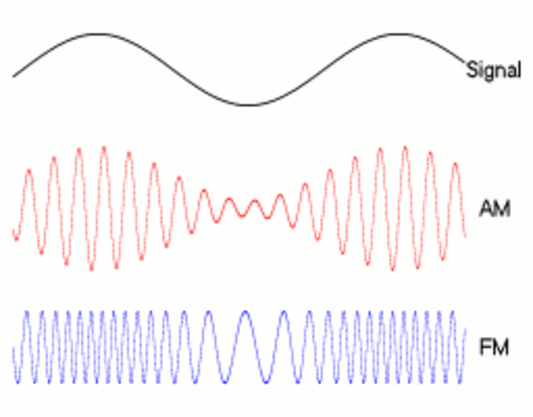
\includegraphics[scale=0.4]{Frequenzaufbereitung/Bilder/Amfm3-en-de.pdf}
% \vspace{-6cm}
%\end{wrapfigure}

\section*{Theorie- und Prüfungsfragen} 


\mucho{1}{TG316}
{Wie wird die folgende Endstufe richtig auf die Sendefrequenz abgestimmt?\\ 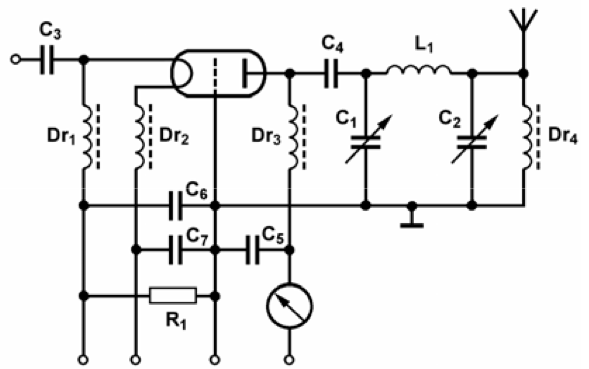
\includegraphics[scale=0.25]{Schaltungstechnik/Bilder/TG313.png}}%Frage
{C1 und C2 auf minimale Kapazität stellen. C2 auf Dip im Anodenstrom (Resonanz) stellen, dann mit C1 einen etwas höheren Anodenstrom einstellen (Leistung auskoppeln). Vorgang mit C1 und C2 wechselweise mehrmals wiederholen bis die maximale Ausgangsleistung erreicht ist. Nach dem Abstimmvorgang sollte ein Dip von etwa 20 $\%$ verbleiben.}%A
{C1 und C2 auf maximale Kapazität stellen. C1 auf Dip im Anodenstrom (Resonanz) stellen, dann mit C2 einen etwas höheren Anodenstrom einstellen (Leistung auskoppeln). Vorgang mit C1 und C2 wechselweise mehrmals wiederholen bis die maximale Ausgangs- leistung erreicht ist. Nach dem Abstimmvorgang sollte ein Dip von etwa 10 $\%$ verbleiben.}%B
{C1 und C2 auf maximale Kapazität stellen. C1 auf Dip im Anodenstrom (Resonanz) stellen, dann mit C2 einen etwas niedrigeren Anodenstrom einstellen (Leistung einkoppeln). Vorgang mit C1 und C2 wechselweise mehrmals wiederholen bis die maximale Oberwellenleistung erreicht ist. Nach dem Abstimmvorgang sollte ein Dip von etwa 10 $\%$ verbleiben.}%C
{C1 und C2 auf minimale Kapazität stellen. C2 auf maximalen Anodenstrom (Resonanz) stellen, dann mit C1 einen etwas niedrigeren Anodenstrom (Dip) einstellen. Vorgang so oft wiederholen bis die maximale Ausgangsleistung erreicht ist. Nach dem Abstimmvorgang sollte ein Dip von etwa 20 $\%$ verbleiben.}%D
{B}%Lösung

\mucho{2}{TG312}
{Welche der nachfolgenden Aussagen trifft nicht(!) für die Schaltung zu?\\ 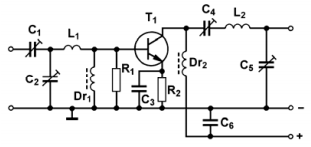
\includegraphics[scale=0.6]{Schaltungstechnik/Bilder/TG311.png}}%Frage
{HF-Eingang und HF-Ausgang sind gleichspannungsfrei.}%A
{C4, C5 und L2 passen den Transistorausgang an die niederohmigere Ausgangsimpedanz an.}%B
{C1, C2 und L1 passen die hochohmigere Eingangsimpedanz an den Transistoreingang an.}%C
{R1 dient zur Arbeitspunkteinstellung des Transistors T1.}%D
{D}%Lösung

\mucho{3}{TG222}
{Bei dieser Schaltung handelt es sich um einen\\ 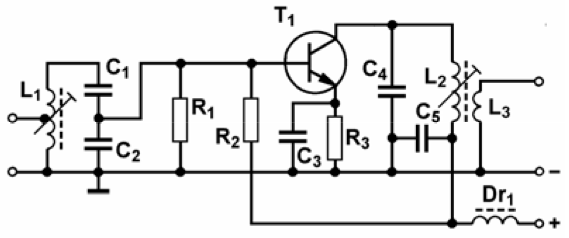
\includegraphics[scale=0.25]{Schaltungstechnik/Bilder/TG222.png}}%Frage
{Oszillator.}%A
{Mischer.}%B
{NF-Verstärker.}%C
{HF-Verstärker.}%D
{D}%Lösung

\mucho{4}{TJ601}
{Welches Gerät ist hier dargestellt?\\ 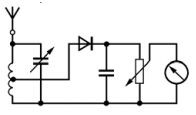
\includegraphics[scale=0.5]{Schaltungstechnik/Bilder/TJ601.png}}%Frage
{Interferenzwellenmesser}%A
{Dipmeter}%B
{Stehwellenmessgerät}%C
{Absorptionsfrequenzmesser}%D
{D}%Lösung

\mucho{5}{TD306}
{Welche Aussage enthält die richtige Beschreibung der Funktionsweise der Regelung in diesem Netzteil, wenn die Ausgangsspannung bei Belastung absinkt?\\ 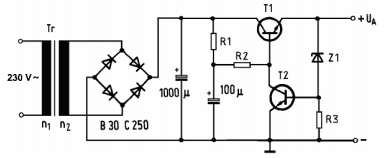
\includegraphics[scale=0.6]{Schaltungstechnik/Bilder/TD306.png}}%Frage
{Sinkt die Ausgangsspannung, so erhält Transistor T2 über die Zenerdiode Z1 weniger Strom und leitet dadurch weniger. Durch den vermindernden Kollektrostrom von T2 verringert sich der Spannungsabfall an R1/R2 und die Basisspannung von T1 steigt und somit auch die Emitterspannung.}%A
{Sinkt die Ausgangsspannung bei Belastung, so erhält Transistor T2 über die Z-Diode Z1 mehr Strom und leitet dadurch stärker. Durch den ansteigenden Kollektrostrom von T2 nimmt der Spannungsabfall an R1/R2 zu. Dabei sinkt die Basisspannung von T1 und die Emitterspannung steigt wieder.}%B
{Sinkt die Ausgangsspannung, so fließt durch Transistor T1 weniger Strom. Durch den sich vermindernden Kollektrostrom von T1 steigt aber der Spannungsabfall an R1/R2 und die Basisspannung von T2 über die Z-Diode Z1. Somit steigt auch die Emitterspannung von T1.}%C
{Sinkt die Ausgangsspannung bei Belastung, so fließt durch den Transistor T1 mehr Belastungsstrom. Der Transistor T2 erhält über Z1 weniger Spannung und der Spannungsabfall am Spannungsteiler R1/R2 nimmt zu. Dabei sinkt die Basisspannung von T1 und die Emitterspannung steigt wieder.}%D
{D}%Lösung